%%%%%%%%%%%%%%%%%%%%%%%%%%%%% Define Article %%%%%%%%%%%%%%%%%%%%%%%%%%%%%%%%%%
\documentclass{article}
%%%%%%%%%%%%%%%%%%%%%%%%%%%%%%%%%%%%%%%%%%%%%%%%%%%%%%%%%%%%%%%%%%%%%%%%%%%%%%%

%%%%%%%%%%%%%%%%%%%%%%%%%%%%% Using Packages %%%%%%%%%%%%%%%%%%%%%%%%%%%%%%%%%%
\usepackage[utf8]{inputenc}
\usepackage{float, geometry, graphicx, fancyhdr, color, xcolor}
\usepackage{amssymb, amsthm, amsmath, tikz, pgfplots, comment, wrapfig}
\usepackage{listings, mdframed, lipsum, psfrag, parskip, empheq, subfig, verbatim, pythonhighlight}
\usepackage[english]{babel}
\usepackage[breaklinks]{hyperref}
\usepackage{titlesec, cite, hyperref, wrapfig, booktabs, bookmark, pdfpages, lastpage, subfloat}
\usepackage{upgreek}
\usepackage{multirow}

%%%%%%%%%%%%%%%%%%%%%%%%%%%%%%%%%%%%%%%%%%%%%%%%%%%%%%%%%%%%%%%%%%%%%%%%%%%%%%%

%%%%%%%%%%%%%%%%%%%%%%%%%% C Code Listing Settings %%%%%%%%%%%%%%%%%%%%%%%%%%%%%%%%%%%%%%%
\definecolor{mGreen}{rgb}{0.25,0.63,0.15}
\definecolor{mGray}{rgb}{0.5,0.5,0.5}
\definecolor{mPurple}{rgb}{0.58,0,0.82}
\definecolor{codeBlue}{rgb}{0.01, 0.2, 0.92}
\definecolor{codegray}{rgb}{0.5,0.5,0.5}
\definecolor{codepurple}{rgb}{0.58,0,0.82}
\definecolor{codeblue}{rgb}{0.13,0.29,0.53}
\definecolor{backgroundColour}{rgb}{0.95,0.95,0.95}

\lstset{
    language=Python,
    backgroundcolor=\color{backgroundColour},
    basicstyle=\ttfamily\small,
    commentstyle=\color{deepGreen},
    keywordstyle=\color{blue},
    numberstyle=\tiny\color{mGray},
    stringstyle=\color{red},
    breakatwhitespace=false,         
    breaklines=true,                 
    captionpos=b,                    
    keepspaces=true,                 
    numbers=left,                    
    numbersep=5pt,                  
    showspaces=false,                
    showstringspaces=false,
    showtabs=false,                  
    tabsize=2,
    frame=single
}

%%%%%%%%%%%%%%%%%%%%%%%%%%%%%%%%%%%%%%%%%%%%%%%%%%%%%%%%%%%%%%%%%%%%%%%%%%%%%%%

% Other Settings
\hypersetup{
    colorlinks = true,
    linkcolor = black,
    urlcolor = blue,
}
\urlstyle{same}

%%%%%%%%%%%%%%%%%%%%%%%%%% Page Setting %%%%%%%%%%%%%%%%%%%%%%%%%%%%%%%%%%%%%%%
\geometry{a4paper}
\pagestyle{fancy}
\fancyhead{}
\fancyhead[L]{Software Engineering}
\fancyhead[C]{Project - Report}
\fancyhead[R]{PAWSTrack}
\fancyfoot{}
\fancyfoot[C]{\thepage \;of \pageref{LastPage}}

%%%%%%%%%%%%%%%%%%%%%%%%%% Define some useful colors %%%%%%%%%%%%%%%%%%%%%%%%%%
\definecolor{ocre}{RGB}{243,102,25}
\definecolor{mygray}{RGB}{243,243,244}
\definecolor{deepGreen}{RGB}{26,111,0}
\definecolor{shallowGreen}{RGB}{235,255,255}
\definecolor{deepBlue}{RGB}{61,124,222}
\definecolor{shallowBlue}{RGB}{235,249,255}
%%%%%%%%%%%%%%%%%%%%%%%%%%%%%%%%%%%%%%%%%%%%%%%%%%%%%%%%%%%%%%%%%%%%%%%%%%%%%%%

%%%%%%%%%%%%%%%%%%%%%%%%%% Define an orangebox command %%%%%%%%%%%%%%%%%%%%%%%%
\newcommand\orangebox[1]{\fcolorbox{ocre}{mygray}{\hspace{1em}#1\hspace{1em}}}
%%%%%%%%%%%%%%%%%%%%%%%%%%%%%%%%%%%%%%%%%%%%%%%%%%%%%%%%%%%%%%%%%%%%%%%%%%%%%%%

%%%%%%%%%%%%%%%%%%%%%%%%%%%% English Environments %%%%%%%%%%%%%%%%%%%%%%%%%%%%%
\newtheoremstyle{mytheoremstyle}{3pt}{3pt}{\normalfont}{0cm}{\rmfamily\bfseries}{}{1em}{{\color{black}\thmname{#1}~\thmnumber{#2}}\thmnote{\,--\,#3}}
\newtheoremstyle{myproblemstyle}{3pt}{3pt}{\normalfont}{0cm}{\rmfamily\bfseries}{}{1em}{{\color{black}\thmname{#1}~\thmnumber{#2}}\thmnote{\,--\,#3}}
\theoremstyle{mytheoremstyle}
\newmdtheoremenv[linewidth=1pt,backgroundcolor=shallowGreen,linecolor=deepGreen,leftmargin=0pt,innerleftmargin=20pt,innerrightmargin=20pt,]{theorem}{Theorem}[section]
\theoremstyle{mytheoremstyle}
\newmdtheoremenv[linewidth=1pt,backgroundcolor=shallowBlue,linecolor=deepBlue,leftmargin=0pt,innerleftmargin=20pt,innerrightmargin=20pt,]{definition}{Definition}[section]
\theoremstyle{myproblemstyle}
\newmdtheoremenv[linecolor=black,leftmargin=0pt,innerleftmargin=10pt,innerrightmargin=10pt,]{problem}{Problem}[section]
%%%%%%%%%%%%%%%%%%%%%%%%%%%%%%%%%%%%%%%%%%%%%%%%%%%%%%%%%%%%%%%%%%%%%%%%%%%%%%%

\title{{\huge \textbf{Habib University \\ Software Engineering - CS/CE 353/374}}

\vspace*{5mm}
{\LARGE \textbf{Project - Report} \\ \textbf{PAWSTrack}} \\
{
\includegraphics[width=0.70\linewidth]{images/logo.png}} \\ 
{\Large \textbf{Instructor:} Abdul Rahman Qaim}}
\author{Lyeba Abid - la07309 \\ Iqra Ahmed - ia07674 \\ Ali Muhammad Asad - aa07190 \\ Sadiqah Mushtaq sm07152}
\date{}

\pgfplotsset{compat=1.18}

\begin{document}
\maketitle

\newpage
\tableofcontents

\newpage
\section{Project Aims, Objectives and Abstract}
PAWSTrack is a web-based shelter pet and record management system developed for the local shelter "PAWS" that is run by our own RA, Ahmed Bilal. Currently, the shelter does not have any proper management system, running and working purely on the efforts of some individuals who are managing the shelter. The shelter is in need of a system that can help them manage their pet records, inventory, staff, and vet records, and their finances / donations. The general public also has no formal way of contacting the shelter, or understanding their operations apart from their social media pages, which are also not comprehensive or efficient in providing information to the public.

PAWSTrack aims to streamline shelter operations for the shelter admin by providing efficient record keeping, enhancing workflow, and ensuring data security. The system will allow the admin to manage pet records including their adoption status, medical history and records, shelter inventory and stock, staff and vet's working at the shelter. The general public can also register on the web-page to understand more about the shelter operations, view current pets at the shelter either undergoing some medical treatment or if they are up for adoption. The users can also register their pets for treatments, or donate to the shelter out of good will. The app aims to create awareness amongst the general public while providing them with a platform to interact with the shelter. 

Key features include a user-friendly interface, scalability, and robust privacy measures. PAWSTrack serves as an intuitive solution for managing pet records, veterinary services, and inventory, contributing to the overall well-being of the shelter and its furry residents.

\newpage
\section{User Specifications}
We will mainly have two types of users; \textbf{Admin} and \textbf{Client}

\begin{enumerate}
    \item \textbf{Admin Users:} 
    
    These users include the shelter staff, vets, manager / admin or any other person in charge. As the Admin, I should be able to:  \begin{itemize}
        \item upload, and manage (update and delete) pet records, including details about each pet
        \item update adoption status of pets
        \item manage and view inventory stocks
        \item upload and manage information about vets / staff etc
        \item upload and manage pets currently being treated, along with their medical bills and expenditure
        \item upload and manage donations / sponsorships for certain items / pets
        \item manage donations received for the shelter
        \item make day to day updates about any specific user's pets currently being treated        
    \end{itemize}
    \item \textbf{Client Users:} 
    
    As a user I should be able to: \begin{itemize}
        \item create a user account 
        \item login to my user account
        \item manage my own profile including personal information, profile picture
        \item view information about the animals and pets currently at the shelter
        \item view information about the general pet care, environment and information about the shelter
        \item view pets or animals up for adoption, and their history if there is any
        \item access customer support channels for inquiries, or assistance (dedicated help center)
        \item make requests for pet adoptions (through dedicated help center right now)
        \item request for treatment for a pet, or if a stray animal / pet needs to be left at the shelter (through dedicated help center right now)
    \end{itemize}
\end{enumerate}
    % include the general user, and users that are registered and have accounts.

    % As either a \textbf{General User}  or a \textbf{User with an Account}, I should be able to:

    % \begin{itemize}
    %     \item view information about the animals and pets currently at the shelter
    %     \item view information about the general pet care, environment and information about the shelter
    %     \item view pets or animals up for adoption, and their history if there is any
    %     \item make requests for pet adoptions
    %     \item request for treatment for a pet, or if a stray animal / pet needs to be left at the shelter
    %     \item view if there are any pets currently being treated and their medical costs
    %     \item create a user profile if needed
    %     \item make donations (either one time or recurring), either general or to something specific if needed
    %     \item access customer support channels for inquiries, or assistance (dedicated help center)
    % \end{itemize}

    % As a \textbf{User with an Account}, I should be able to:
    % \begin{itemize}
    %     \item create a profile if I don't have one already
    %     \item login to my account
    %     \item manage my own profile, including personal information, profile picture
    %     \item register a pet of my own to the shelter for treatment
    %     \item view day to day status of my own pets left at the shelter for treatment
    %     \item make payments for any expenditure on my pet left at the office
    %     \item leave feedback, reviews, comments and ratings for the shelter's services, and experience with the shelter
    % \end{itemize}


\newpage
\section{System Specifications}
\begin{enumerate}
    \item \textbf{Admin Management} \begin{enumerate}
        \item \textit{Admin Registration} (only done by another admin) \begin{enumerate}
            \item Username
            \item Email
            \item Password
        \end{enumerate}
        \item \textit{Admin Login} \begin{enumerate}
            \item Username
            \item Password
        \end{enumerate}
        \item \textit{Account Management} \begin{enumerate}
            \item Add / Edit profile picture
            \item Change password
            \item Change email
        \end{enumerate}
    \end{enumerate}
    \item \textbf{User Account Management} \begin{enumerate}
        \item \textit{User Registration} \begin{enumerate}
            \item Username
            \item Email
            \item Password
        \end{enumerate}
        \item \textit{User Login} \begin{enumerate}
            \item Username
            \item Password
        \end{enumerate}
        \item \textit{Account Management} \begin{enumerate}
            \item Add / Edit profile picture
            \item Change password
            \item Change email
        \end{enumerate}
    \end{enumerate}
    \item \textbf{Dashboard} \begin{enumerate}
        \item \textit{Admin Dashboard} \begin{enumerate}
            \item View and manage pet records
            \item View and manage user messages
            \item add or remove staff
        \end{enumerate}
        \item \textit{User Dashboard} \begin{enumerate}
            \item View and edit personal details
            \item View animals and pets at the shelter
            \item View shelter information (about us page) to understand shelter operations
            \item Contact customer support by leaving a message through the ``Contact Us'' page
        \end{enumerate}
    \end{enumerate}
    \item \textbf{Pet Management (Admin Only)} \begin{enumerate}
        \item \textit{Add new pet profiles} \begin{enumerate}
            \item Picture
            \item Name
            \item Age
            \item Type
            \item Adoption status
            \item Adoption history
            \item Medical history
            \item Treatment status
            \item Treatment history
            \item Treatment cost
            \item Living status (dead or alive)
        \end{enumerate}
        \item Update / edit existing pet profiles
        \item Delete pet profiles 
    \end{enumerate}
    \item \textbf{Customer Support Management (Users)} \begin{enumerate}
        \item \textit{User can contact shelter by leaving a message} \begin{enumerate}
            \item Name
            \item Email
            \item Phone
            \item Subject
            \item Message details / query / concern / request 
        \end{enumerate}
        \item User can contact shelter through telephone
        \item User can visit the shelter by following the location given on the attached map
    \end{enumerate}
    \item \textbf{Customer Support Management (Admin)} \begin{enumerate}
        \item Admin can view messages left by users
        \item \textit{Admin can respond to messages} \begin{enumerate}
            \item Email
            \item Phone
        \end{enumerate}
    \end{enumerate}
\end{enumerate}

% \begin{enumerate}
%     \item User Management \begin{itemize}
%         \item Register
%         \item Login Page
%         \item Manage Accounts
%     \end{itemize}
%     \item Dashboard (Admin, and Clients): view the above mentioned information, allow searching and relevant information
%     \item Pet management: \begin{itemize}
%         \item manage pet profiles
%         \item upload media
%         \item track medical history
%         \item manage adoption status / applications if needed
%     \end{itemize}  
%     \item Inventory management: \begin{itemize}
%         \item view 
%         \item add
%         \item update 
%         \item delete
%     \end{itemize} 
%     \item Doctor’s Appointment System \begin{itemize}
%         \item Pet details, Condition
%         \item Date time
%         \item Doctor
%     \end{itemize}
%     \item Contact management
%     \item Payment / Donation System: secure payment processing, track donations and financial records, generate receipts, and donation reports.
%     \item Rating / Comment / Review system
% \end{enumerate}

\newpage
\section{Functional and Non-Functional Requirements}
\subsection{Functional Requirements}
\begin{itemize}
    \item Admin Management - can manage accounts
    \item User Account Management
    \item Dashboard - can view relevant details
    \item Pet Management by adding, updating, or deleting pet details
    \item Customer Support Management \begin{itemize}
        \item User can contact the shelter
        \item Admin can respond to user queries and messages
    \end{itemize}
\end{itemize}

\subsection{Non-Functional Requirements}
\begin{itemize}
    \item Web Application only
    \item Performance: system should be able to handle multiple users at the same time without any significant performance degradation
    \item Every request should not take more than 2 seconds to complete
    \item Security: Ensure that users data is secure, and that unauthorized users cannot access admin only details and operations
    \item Usability: System should be user friendly, and easy to navigate by both the admin and the clients
    \item Compatibility: System should be compatible for various kinds of devices - in our case, various browsers
    \item Maintainability: more features can be added without affecting existing ones
    \item Reliability: system should not be down for long periods of time
\end{itemize}

\newpage
\section{Mockups and Wireframes}

\begin{figure}[H]
    \centering
    \begin{tabular}{| c | c |}
        \hline
        \subfloat[Sign-up / Register Screen]{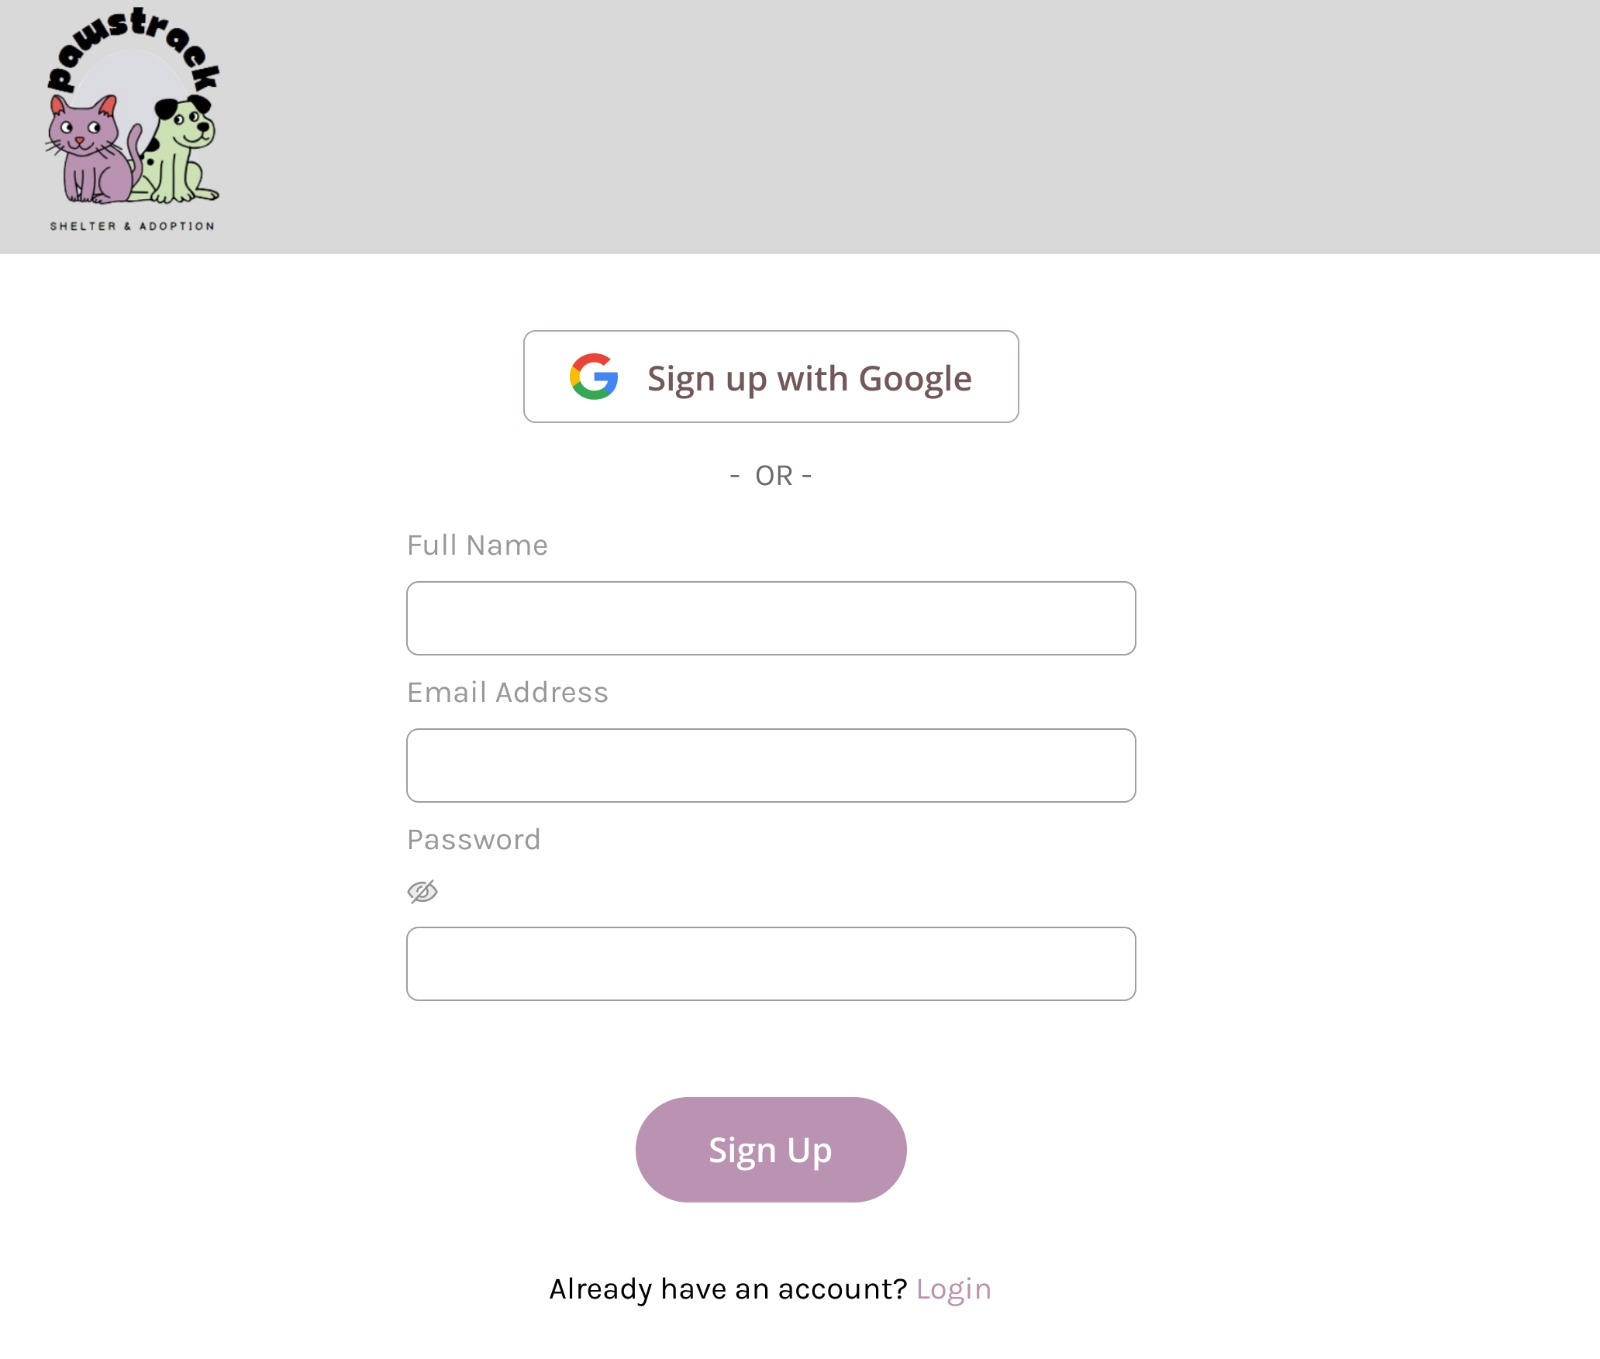
\includegraphics[width=0.45\textwidth]{images/Signup.jpg}} & \subfloat[Login Screen]{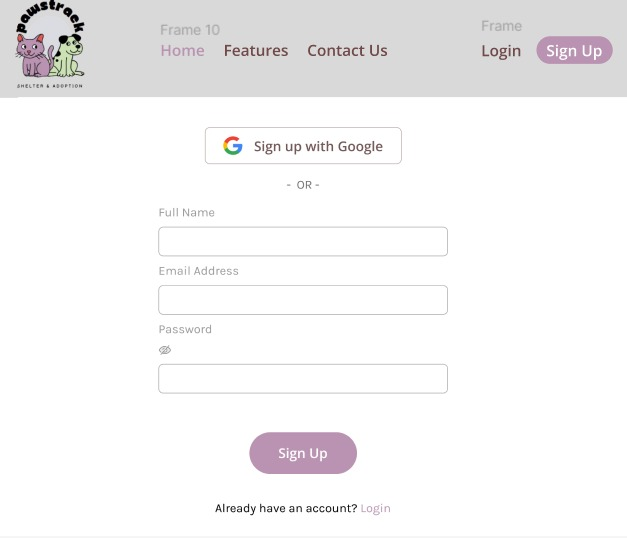
\includegraphics[width=0.45\textwidth]{images/Login.jpg}} \\ \hline
        \subfloat[Account Settings Screen]{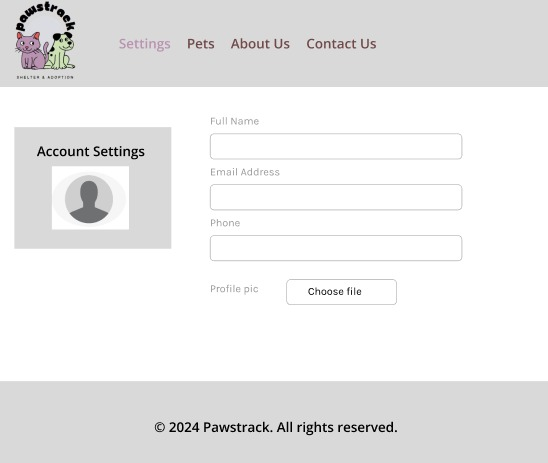
\includegraphics[width=0.45\textwidth]{images/account_settings.png}} & \subfloat[About Us Screen]{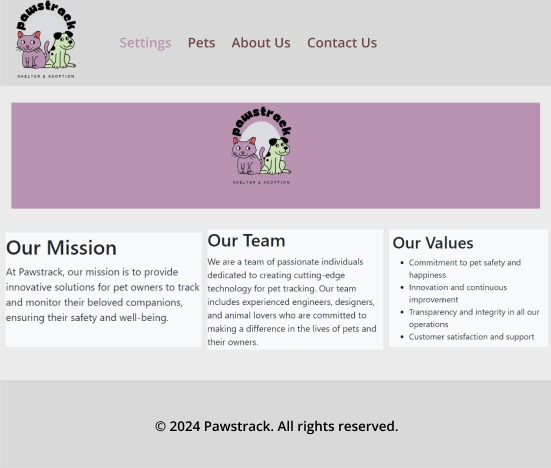
\includegraphics[width=0.45\textwidth]{images/about_us.png}} \\ \hline
        \subfloat[Contact Us Screen]{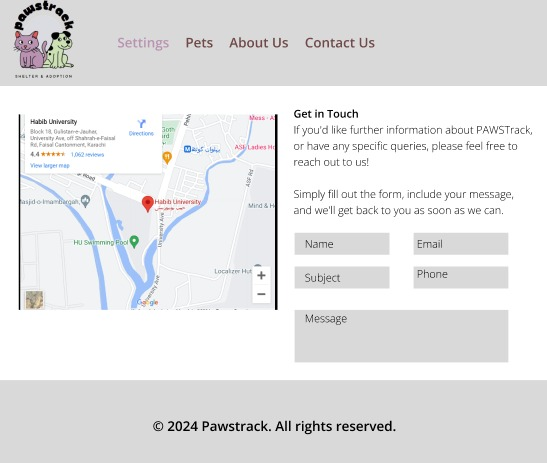
\includegraphics[width=0.45\textwidth]{images/contact_us.png}} & \subfloat[Pet list screen showing all pets]{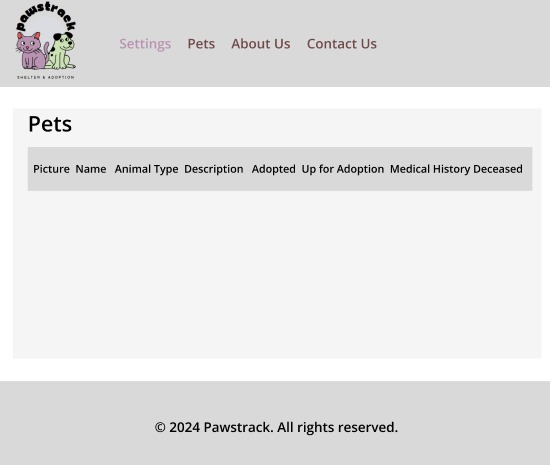
\includegraphics[width=0.45\textwidth]{images/pet_list.png}} \\ \hline
    \end{tabular}
\end{figure}
\begin{figure}[H]
    \centering
    \begin{tabular}{| c | c |}
        \hline
        \subfloat[Pet Details screen showing details of a single pet]{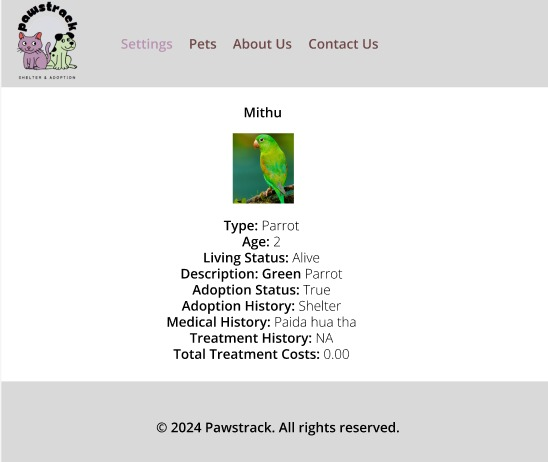
\includegraphics[width=0.45\textwidth]{images/pet_details.png}} & \subfloat[Pet Add and Update Screen]{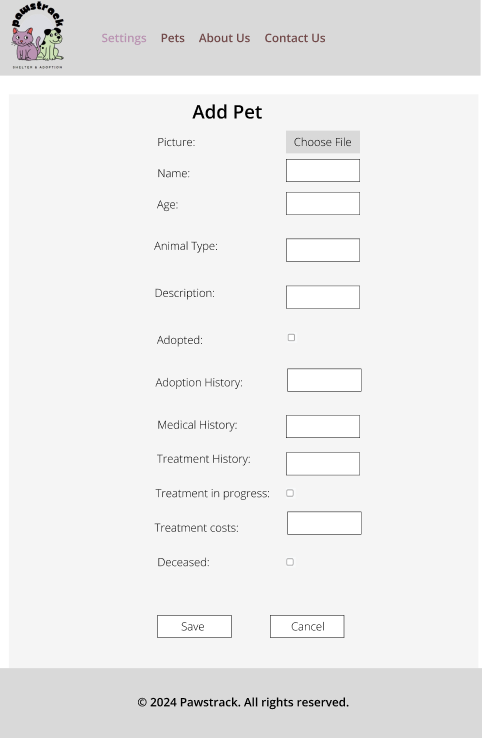
\includegraphics[width=0.45\textwidth]{images/pet_add_update.png}} \\ \hline
        \subfloat[Message list screen]{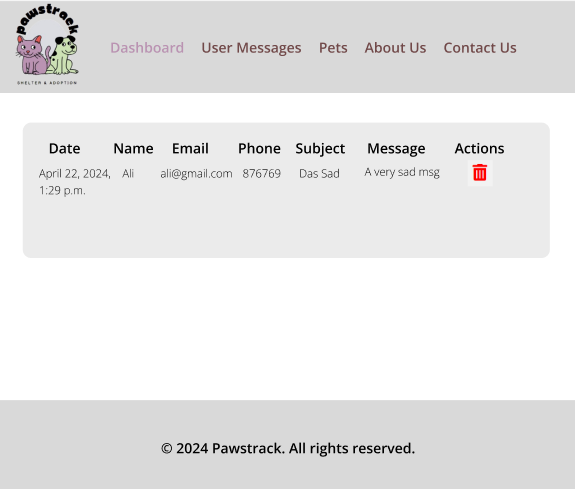
\includegraphics[width=0.45\textwidth]{images/messages.png}} & \subfloat[Confirm delete screen]{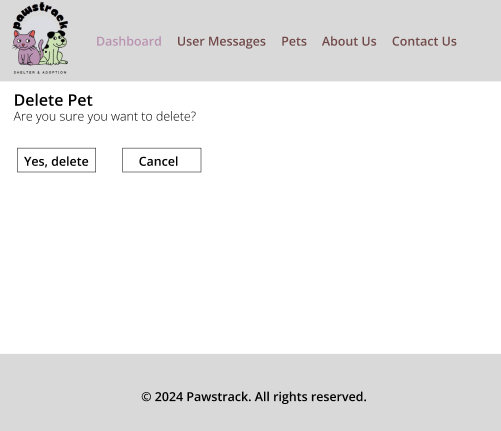
\includegraphics[width=0.45\textwidth]{images/delete.png}} \\ \hline
    \end{tabular}
    \caption{Mockups and Wireframes of the PAWSTrack Web Application}
\end{figure}

The above mockups and wireframes basically show the different screens of the web application. Some screens like the delete screen were reused, the add screen was used to update as well, and some screens are admin only. 
% The first two images show the sign-up and login screens respectively. The third image shows the account settings screen where the user can change their account settings. The fourth image shows the about us screen which gives a brief introduction about the application. The fifth image shows the contact us screen where the user can contact the admin. The sixth image shows the pet list screen where all the pets are displayed. The seventh image shows the pet details screen where the details of a single pet are displayed. The eighth image shows the pet add and update screen where the admin can add or update the pet details. The ninth image shows the message list screen where all the messages are displayed. The last image shows the confirm delete screen where the admin can confirm the deletion of a pet.

\newpage
\section{UML Diagrams}
This section will cover the UML diagrams for the system. The UML diagrams are a visual representation of the system's architecture, design, and functionality, and help in understanding the system's structure and behavior. 

\subsection{Use Cases}
\begin{figure}[htbp]
    \centering
    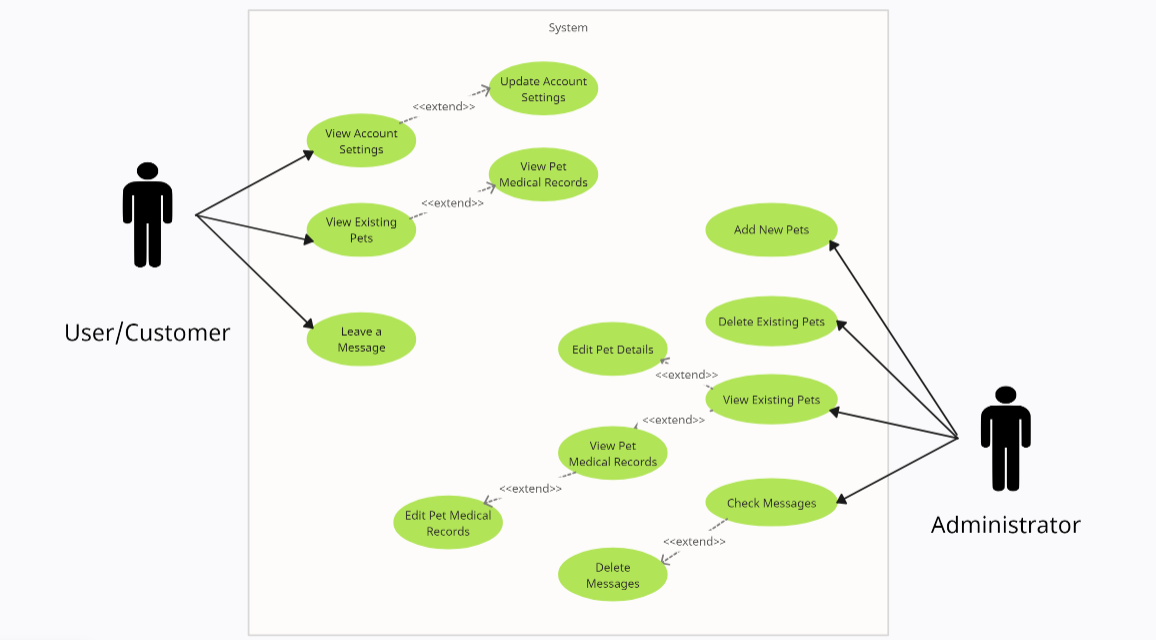
\includegraphics[width=\textwidth]{images/Use Case Diagram.png}
    \caption{Use Case Diagram showing the different use cases of the system.}
\end{figure}

The above Use Case diagram effectively incorporates the different use cases of our system and the actors involved in each use case. The actors are the admin and the user/customer. The admin add new pets, view existing pets which extends to editing their details or medical records which further extends to editing the medical records as we need to be able to manage and update pet records. The admin can also delete a pet. Admin can also check messages, which they can choose to delete. 

The user can view and update their own account, view pets, view existing pets and their details, and contact the shelter. The user can also view the shelter information.

\newpage
\subsection{Sequence Diagram}
Based on the use cases, and provided system specifications, and functional reuqirements, we have created the following sequence diagram which encapsulates the requests / responses made from the system and to the database to fetch required information based on made requests.
\begin{figure}[H]
    \centering
    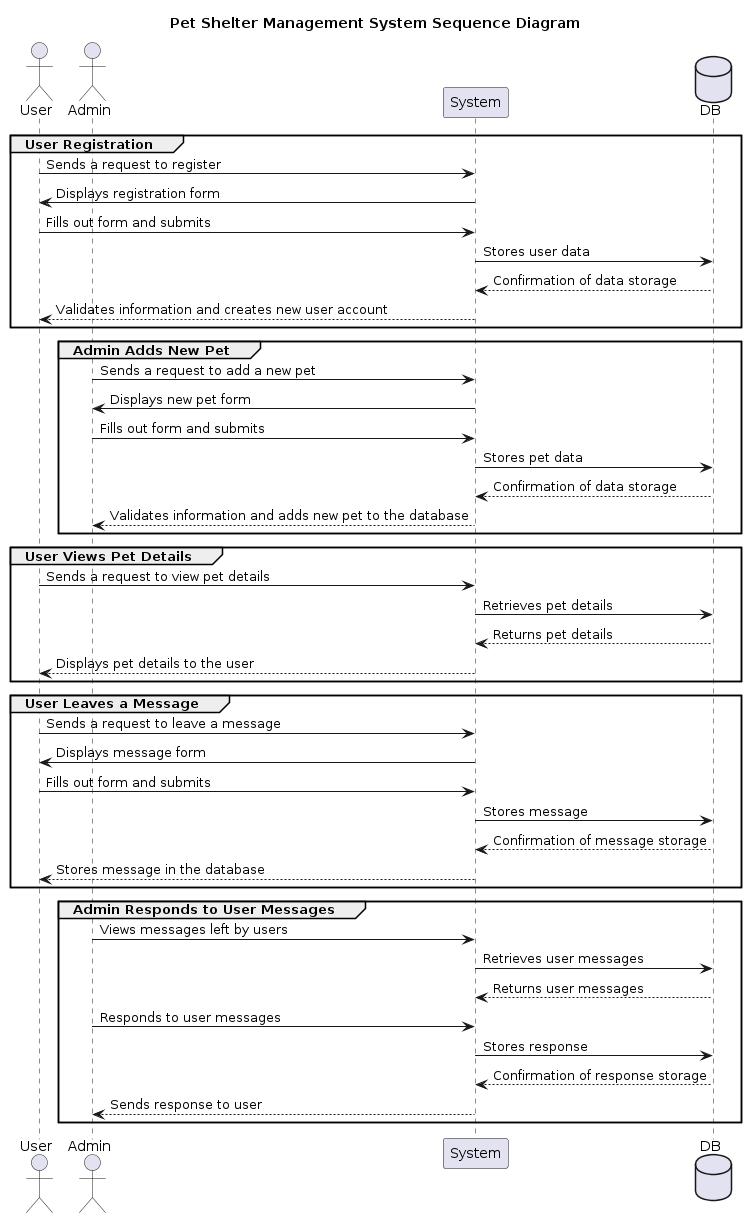
\includegraphics[width=0.7\textwidth]{images/seqDiagram.png}
    \caption{Sequence Diagram showing user/admin-system interaction}
\end{figure}


\subsection{Class Diagram}
\begin{figure}[H]
    \centering
    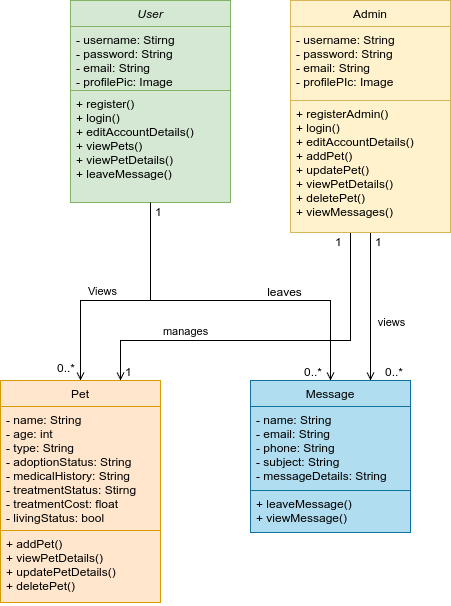
\includegraphics[width=0.8\textwidth]{images/classDiagram.png}
    \caption{Class Diagram showing the different classes and their relationships}
\end{figure}
A user can view multiple pets or a pet can be viewed by multiple users. A user can also leave multiple messages, but a message can only be left by one user. An admin can manage multiple pets, and can also respond to multiple messages.

\subsection{ERD}
\begin{figure}[H]
    \centering
    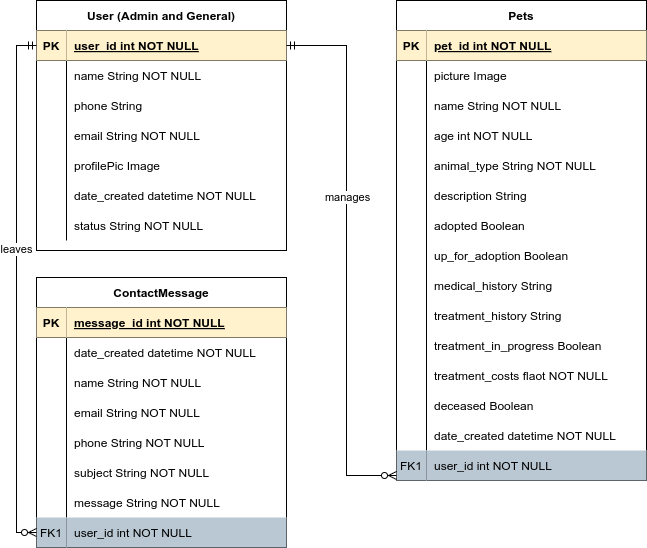
\includegraphics[width=\textwidth]{images/erd.png}
    \caption{Entity Relationship Diagram showing the different entities and their relationships}
\end{figure}
In the above ERD diagram, we represent both the general user and admin by one table since they mostly contain the same information, apart from status which basically tells if the user is an admin or not. Each user has their own unique id. Each user can leave multiple messages, however, one message belongs to only one user, hence we define a one-to-many relationship between the user and message table, with the \verb|user_id| being the foreign key in the message table. Similarly, each pet can be viewed by multiple users, however, there is no relation defined for this since it is not necessary for the system. However, one admin can manage multiple pets, hence we define a one-to-many relationship between the admin and pet table, with the \verb|user_id| being the foreign key in the pet table. Each pet also has a unique \verb|pet_id| associated with it, which is used to identify each pet and display that pet's information. 

\newpage
\subsection{Architecture}
\begin{figure}[htbp]
    \centering
    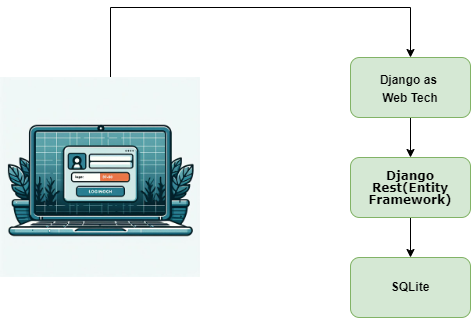
\includegraphics[width=0.85\textwidth]{images/Architecture Diagram.png}
    \caption{Architecture Diagram showing the different components of the system}
\end{figure}
Our architectural diagram is defined as shown above. We have made a web application using the python's Django as our main web technology. With Django, we've used basic HTML, CSS, and JavaScript for implementing various functionalities for the web-pages. For the API calls and handling, we've used Django Rest Framework which is a powerful and flexible toolkit for building Web APIs, efficiently handling the requests and responses. Our data is being stored in a SQLite database, a lightweight file based database which is easy to use and manage. 

%%%%%%%%%%% Sequence Diagram PlantUML Script %%%%%%%%%%%
% @startuml
% actor User
% actor Admin
% participant System
% database DB

% title Pet Shelter Management System Sequence Diagram

% group User Registration
% User -> System : Sends a request to register
% System -> User : Displays registration form
% User -> System : Fills out form and submits
% System -> DB : Stores user data
% DB --> System : Confirmation of data storage
% System --> User : Validates information and creates new user account
% end

% group Admin Adds New Pet
% Admin -> System : Sends a request to add a new pet
% System -> Admin : Displays new pet form
% Admin -> System : Fills out form and submits
% System -> DB : Stores pet data
% DB --> System : Confirmation of data storage
% System --> Admin : Validates information and adds new pet to the database
% end

% group User Views Pet Details
% User -> System : Sends a request to view pet details
% System -> DB : Retrieves pet details
% DB --> System : Returns pet details
% System --> User : Displays pet details to the user
% end

% group User Leaves a Message
% User -> System : Sends a request to leave a message
% System -> User : Displays message form
% User -> System : Fills out form and submits
% System -> DB : Stores message
% DB --> System : Confirmation of message storage
% System --> User : Stores message in the database
% end

% group Admin Responds to User Messages
% Admin -> System : Views messages left by users
% System -> DB : Retrieves user messages
% DB --> System : Returns user messages
% Admin -> System : Responds to user messages
% System -> DB : Stores response
% DB --> System : Confirmation of response storage
% System --> Admin : Sends response to user
% end
% @enduml

\newpage
\section{Requirement Traceablity Matrix}

\begin{table}[htbp]
\centering
\renewcommand{\arraystretch}{1.4}
% \caption{Requirement Traceability Matrix}
\begin{tabular}{|c|p{3cm}|p{2cm}|p{6cm}|}
\hline
\textbf{S.No} & \textbf{Module Name} & \textbf{Applicable Roles} & \textbf{Description} \\
\hline
\multirow{3}{*}{1} & \multirow{3}{=}{Admin Management} & \multirow{3}{=}{Admin} & Admin can register \\
 &  &  & Admin can login \\
 &  &  & Admin can manage account \\
\hline
\multirow{3}{*}{2} & \multirow{3}{=}{User Account Management} & \multirow{3}{=}{User} & User can register \\
 &  &  & User can login \\
 &  &  & User can manage account \\
\hline
\multirow{4}{*}{3} & \multirow{4}{=}{Dashboard} & \multirow{3}{=}{Admin} & Admin can view and manage pet records \\
 &  &  & Admin can view and manage user messages \\
 &  &  & Admin can add or remove staff \\
\cline{3-4}
 &  & \multirow{4}{=}{User}  & User can view and edit personal details \\
 &  &  & User can view animals and pets at the shelter \\
 &  &  & User can view shelter information \\
 &  &  & User can contact customer support \\
\hline
\multirow{3}{*}{4} & \multirow{3}{=}{Pet Management} & \multirow{2}{=}{Admin} & Admin can add new pet profiles \\
 &  &  & Admin can update or edit existing pet profiles \\
 &  &  & Admin can delete pet profiles \\
\hline
\multirow{4}{*}{5} & \multirow{4}{=}{Customer Support Management} & \multirow{2}{=}{Admin} & Admin can view messages left by users \\
 &  &  & Admin can respond to messages \\
\cline{3-4}
 &  & \multirow{2}{=}{User} & User can contact shelter by leaving a message \\
 &  &  & User can contact shelter through telephone \\
\hline
\end{tabular}
\end{table}





\newpage
\section{DevOps User Stories, and Acceptance Criteria}
\subsection{Admin Stories}
\subsubsection*{1. As an Admin, I can make daily updates on pets}
\textbf{Description:} As an Admin, I want to make day-to-day updates about pets currently being held at the shelter. This can include their daily pictures, wallpapers, their treatment if any, their livelihood, their adoption status, new animals, etc.

\textbf{Acceptance Criteria:}
\begin{enumerate}
    \item \textbf{Pet Updates:}
    \begin{itemize}
        \item Admin can upload one picture per pet profile daily.
        \item Mandatory fields (name, species, breed, age, gender, ID) are accurately populated and give errors if wrong data types are used for specific fields.
        \item Treatment information and adoption status are correctly displayed for each pet.
    \end{itemize}
    
    \item \textbf{Livelihood Updates:}
    \begin{itemize}
        \item Admin can post updates on pets' general well-being.
        \item Updates include behavior, interactions, and special needs.
    \end{itemize}
    
    \item \textbf{Adoption Status Updates:}
    \begin{itemize}
        \item Admin can update adoption status (available, pending, adopted) for each pet.
        \item Users can view real-time adoption status changes on pet profiles.
    \end{itemize}
    
    \item \textbf{New Arrivals Updates:}
    \begin{itemize}
        \item Admin promptly adds profiles for new animals.
        \item Correctly captures species, breed, age, and gender for each new arrival.
        \item Includes at least one picture for each new arrival.
    \end{itemize}
\end{enumerate}

\subsubsection*{2. As an Admin, I can manage detailed pet records}
\textbf{Description:} As an Admin, I want the ability to upload and manage detailed records for each pet. This includes uploading images, maintaining a comprehensive medical history, and updating the adoption status. Efficient pet record management ensures accurate information about each animal in the shelter.

\textbf{Acceptance Criteria:}
    \begin{enumerate}
    \item There should be an option to add a new pet.
    \item No record should be created without a pet name.
    \item No record should be created without specifying the pet type.
    \item No record should be created without providing pet description, history, and setting an adoption status.
    \item It should be possible to create a record without uploading a pet image.
    \item The submit button should successfully create a pet record when clicked.
    \item Pet records should be editable.
    \item Pet records should be deletable.
\end{enumerate}

\subsubsection*{3. As an Admin, I can manage pet treatments}
\textbf{Description:} As an Admin, I want to upload and manage information about pets currently undergoing treatment. This includes tracking medical bills and expenditures associated with the treatment. Efficient management of treatment records is essential for providing optimal care to the animals.

\textbf{Acceptance Criteria:}
\begin{enumerate}
    \item Add a pet to the treatment page.
    \item Add the vet treating the pet to the treatment page.
    \item Add a description about the treatment.
    \item Add medication for the treatment.
    \item Add day-to-day cost for the treatment.
    \item If the cost is covered, the total cost should be updated accordingly.
\end{enumerate}

\subsubsection*{4. As an Admin, I can manage adoption status and history}
\textbf{Description:} As an Admin, I want the capability to update the adoption status of pets and track adoption applications efficiently. This functionality is crucial for managing the adoption process, ensuring transparency, and matching pets with suitable adopters.

\textbf{Acceptance Criteria:}
\begin{enumerate}
    \item A pet can be added without any adoption history.
    \item It should be possible to set adoption status for any pet successfully.
    \item Adoption history can be updated successfully.
    \item Adoption status and history should be successfully displayed.
\end{enumerate}

\subsubsection*{5. As an Admin, I can manage inventory stocks}
\textbf{Description:} As an Admin, I want to manage and view inventory stocks easily. This involves the ability to add, update, or delete stock items as needed. Efficient inventory management ensures the availability of necessary supplies for the shelter's operations.

\textbf{Acceptance Criteria:}
\begin{enumerate}
    \item Add inventory items.
    \item Add inventory item details.
    \item Add inventory item quantity.
    \item Add inventory item price.
    \item Add inventory item shelf-life if needed.
    \item Update inventory item quantity/price as needed.
    \item Delete an inventory item.
\end{enumerate}


\subsubsection*{6. As an Admin, I can maintain vets and staff information}
\textbf{Description:} As an Admin, I want to upload and manage information about vets and staff members, including their roles and responsibilities within the shelter. This functionality ensures that the team's details are organized and accessible for efficient collaboration.

\textbf{Acceptance Criteria:}
\begin{enumerate}
    \item Admin should be allowed to update the vet's information.
    \item A new vet cannot be left nameless, or without a description or contact information.
    \item Information about the vet should be displayed correctly.
\end{enumerate}

\subsubsection*{7. As an Admin, I can manage pet treatments}
\textbf{Description:} As an Admin, I want to upload and manage information about pets currently undergoing treatment. This includes tracking medical bills and expenditures associated with the treatment. Efficient management of treatment records is essential for providing optimal care to the animals.

\textbf{Acceptance Criteria:}
\begin{enumerate}
    \item Add a pet to the treatment page.
    \item Add the vet treating the pet.
    \item Add a description about the treatment.
    \item Add medication for the treatment.
    \item Add day-to-day cost for the treatment.
    \item If the cost is covered, the total cost should be updated accordingly.
\end{enumerate}

\subsubsection*{8. As an Admin, I can login to dashboard securely:}
\textbf{Description:}As an Admin, I want to securely log in to the system to access the admin dashboard and perform various administrative tasks. This includes ensuring that only authorized personnel can access sensitive information and functionalities.

\textbf{Acceptance Criteria:}
\begin{enumerate}
    \item Admin ID should be unique.
    \item The system should deny access if the credentials are incorrect.
    \item The system should allow access if the credentials are correct.
    \item Try to login with only username, and only password.
\end{enumerate}

\subsubsection*{9. As an Admin, I can manage donations and sponsorships}
\textbf{Description:} As an Admin, I want to handle and manage donations and sponsorships for items or specific pets. This involves keeping track of received donations and ensuring transparency in financial transactions related to the shelter's operations.

\textbf{Acceptance Criteria:}
\begin{enumerate}
    \item A donor or sponsor should be able to contact via customer support.
    \item A donation or sponsorship should be logged into the system and linked to the pet or inventory if needed.
    \item Donor details should be successfully displayed.
    \item Sponsor details should be successfully displayed.
    \item Donation amount/sponsorship amount should be updated.
\end{enumerate}


\subsection{User Stories}
\subsubsection*{1. As a User, I can view adoption candidates} 
    \textbf{Description:} As a General User, I want to view pets or animals available for adoption and their history, if available, to make informed adoption decisions. 
    
    \textbf{Acceptance Criteria:}
    \begin{itemize}
       \item System should successfully display list of pets available for adoption.
       \item On selecting to view a pet, the adoption status should display if the pet is available or not.
       \item The adoption history and relevant details about the pet should be displayed.
    \end{itemize}
    
\subsubsection*{2. As a User, I can access customer support} 
    \textbf{Description:} As a User with an Account, I want to access customer support channels for inquiries or assistance, such as a dedicated help center or information section, so that I can seek help or a clarification whenever needed. 
    
    \textbf{Acceptance Criteria:}
    \begin{itemize}
        \item Provide customer service to customers.
        \item Provide contact information about the team/shelter.
        \item Working email channel.
        \item Allow message box on the page.
        \item User notified when their query is sent.
    \end{itemize}
    
\subsubsection*{3. As a User, I can understand Shelter operations} 
    \textbf{Description:} As a General User, I want to view information about general pet care, the shelter environment, and relevant information to better understand the shelter’s operations. 

    \textbf{Acceptance Criteria:}
    \begin{itemize}
       \item Provide customer service to customers.
       \item Provide contact information about the team/shelter.
       \item Working email channel.
       \item Allow message box on the page.
       \item User notified when their query is sent.
    \end{itemize}
    
\subsubsection*{4. As a User, I can login to my account and manage it} 
    \textbf{Description:} As a user with an account, I want to be able to manage my account details, such as name, password, email, contact number, and track my pets etc. 
    
    \textbf{Acceptance Criteria:}
    \begin{itemize}
        \item Authenticate the user's credentials.
        \item Try logging in with only username, and with only password.
        \item Forget password button.
        \item Try logging in with incorrect credentials.
        \item Update username.
        \item Update password.
        \item Update account picture.
        \item Update further details.
        \item Update pets.
        \item View and track pets.
    \end{itemize}
    
\subsubsection*{5. As a User, I can create my account} 
    
    \textbf{Description:} As a User with an Account, I want to create my account, including personal information such as email, username, password, so that I can personalize my experience on the platform. 
    
    \textbf{Acceptance Criteria:}
    \begin{itemize}
       \item UserID must be unique.
       \item Authenticate user credentials.
       \item Try registering with duplicate credentials.
       \item Try registering with only email, or username, or password.
       \item Try registering with invalid password.
       \item Allow access if account created.
    \end{itemize}

\subsubsection*{6. As a User, I can register and track my pet} 
     
    \textbf{Description:} As a User with an Account, I want to register my own pet to the shelter for treatment, track their day-to-day status, and make payments for any associated expenditures, so that I can ensure proper care for my pet. 
    
    \textbf{Acceptance Criteria:}
    \begin{itemize}
       \item Allow user to register a pet. \vspace*{-1mm}
       \item Pet name. \vspace*{-1mm}
       \item Pet type. \vspace*{-1mm}
       \item Pet description. \vspace*{-1mm}
       \item Pet image (optional). \vspace*{-1mm}
       \item Show pet's status. \vspace*{-1mm}
       \item Show pet's medical bills, and history. \vspace*{-1mm}
       \item Allow payment option. \vspace*{-1mm}
    \end{itemize}

\subsubsection*{7. As a User, I can leave my feedback} 
    
    \textbf{Description:} As a User with an Account, I want to leave feedback, reviews, comments, and ratings for the shelter's services and my overall experience, so that I can contribute to improving the shelter's services and share my experience with others. 
    
    \textbf{Acceptance Criteria:}
    \begin{itemize}
       \item Allow the user to leave feedback.
       \item Allow user to give a review and ratings.
       \item Reviews should be displayed correctly.
    \end{itemize}

\subsubsection*{8. As a User, I can make adoption requests} 
    
    \textbf{Description:} As a General User, I want to make requests for pet adoptions easily through the system, so that I can initiate the adoption process conveniently.
    
    \textbf{Acceptance Criteria:}
    \begin{itemize}
      \item Display pets available for adoption.
      \item Request for adoption form/button available for pet.
      \item Notify the user if their adoption request has been sent forward.
      \item Notify user when their request is processed.
    \end{itemize}

\subsubsection*{9. As a User, I can make donations}     
    \textbf{Description:} As a User with an Account, I want to make one-time or recurring donations, either general or specific, through a secure payment processing system, so that I can support the shelter financially and contribute to its cause.
    
    \textbf{Acceptance Criteria:}
    \begin{itemize}
        \item Allow a page where donations can be made via bank or card etc. OTP should be sent to provided contact info.
        \item Receipt should be generated to \item show payment processed successfully.
        \item Receipt should not be generated, an error thrown when not processed.
    \end{itemize}


\newpage
\section{Test Plan}

% \begin{enumerate}
%     \item \textbf{}
%     \begin{itemize}
%         \item \textbf{Test Case 1:}
%         \begin{itemize}
%             \item \textbf{Steps:}
%             \begin{enumerate}
%                 \item
%             \end{enumerate}
%             \item \textbf{Expected Result:}
%         \end{itemize}
%         \item \textbf{Test Case 2:}
%         \begin{itemize}
%             \item \textbf{Steps:}
%             \begin{enumerate}
%                 \item
%             \end{enumerate}
%             \item \textbf{Expected Result:}
%         \end{itemize}
%         \item \textbf{Test Case 3:}
%         \begin{itemize}
%             \item \textbf{Steps:}
%             \begin{enumerate}
%                 \item
%             \end{enumerate}
%             \item \textbf{Expected Result:}
%         \end{itemize}
%     \end{itemize}
%     \item \textbf{}
%     \begin{itemize}
%         \item \textbf{Test Case 4:}
%         \begin{itemize}
%             \item \textbf{Steps:}
%             \begin{enumerate}
%                 \item
%             \end{enumerate}
%             \item \textbf{Expected Result:}
%         \end{itemize}
%     \end{itemize}
%     \item \textbf{}
%     \begin{itemize}
%         \item \textbf{Test Case 5:}
%         \begin{itemize}
%             \item \textbf{Steps:}
%             \begin{enumerate}
%                 \item
%             \end{enumerate}
%             \item \textbf{Expected Result:}
%         \end{itemize}
%         \item \textbf{Test Case 6:}
%         \begin{itemize}
%             \item \textbf{Steps:}
%             \begin{enumerate}
%                 \item
%             \end{enumerate}
%             \item \textbf{Expected Result:}
%         \end{itemize}
%         \item \textbf{Test Case 7:}
%         \begin{itemize}
%             \item \textbf{Steps:}
%             \begin{enumerate}
%                 \item
%             \end{enumerate}
%             \item \textbf{Expected Result:}
%         \end{itemize}
%         \item \textbf{Test Case 8:}
%         \begin{itemize}
%             \item \textbf{Steps:}
%             \begin{enumerate}
%                 \item
%             \end{enumerate}
%             \item \textbf{Expected Result:}
%         \end{itemize}
%         \item \textbf{Test Case 9:}
%         \begin{itemize}
%             \item \textbf{Steps:}
%             \begin{enumerate}
%                 \item
%             \end{enumerate}
%             \item \textbf{Expected Result:}
%         \end{itemize}
%     \end{itemize}
%     \item \textbf{}
%         \begin{itemize}
%         \item \textbf{Test Case 10:}
%         \begin{itemize}
%             \item \textbf{Steps:}
%             \begin{enumerate}
%                 \item
%             \end{enumerate}
%             \item \textbf{Expected Result:}
%         \end{itemize}
%         \item \textbf{Test Case 11:}
%         \begin{itemize}
%             \item \textbf{Steps:}
%             \begin{enumerate}
%                 \item
%             \end{enumerate}
%             \item \textbf{Expected Result:}
%         \end{itemize}
%         \item \textbf{Test Case 12:}
%         \begin{itemize}
%             \item \textbf{Steps:}
%             \begin{enumerate}
%                 \item
%             \end{enumerate}
%             \item \textbf{Expected Result:}
%         \end{itemize}
%     \end{itemize}
%     \item \textbf{}
%         \begin{itemize}
%         \item \textbf{Test Case 13:}
%         \begin{itemize}
%             \item \textbf{Steps:}
%             \begin{enumerate}
%                 \item
%             \end{enumerate}
%             \item \textbf{Expected Result:}
%         \end{itemize}
%         \item \textbf{Test Case 14:}
%         \begin{itemize}
%             \item \textbf{Steps:}
%             \begin{enumerate}
%                 \item
%             \end{enumerate}
%             \item \textbf{Expected Result:}
%         \end{itemize}
%         \item \textbf{Test Case 15:}
%         \begin{itemize}
%             \item \textbf{Steps:}
%             \begin{enumerate}
%                 \item
%             \end{enumerate}
%             \item \textbf{Expected Result:}
%         \end{itemize}
%     \end{itemize}
%     \item \textbf{}
%         \begin{itemize}
%         \item \textbf{Test Case 16:}
%         \begin{itemize}
%             \item \textbf{Steps:}
%             \begin{enumerate}
%                 \item
%             \end{enumerate}
%             \item \textbf{Expected Result:}
%         \end{itemize}
%     \end{itemize}
% \end{enumerate}

\begin{enumerate}
    \item \textbf{Admin Registration and Login:}
    \begin{itemize}
        \item \textbf{Test Case 1:} Test admin registration with valid credentials.
        \begin{itemize}
            \item \textbf{Steps:}
            \begin{enumerate}
                \item Navigate to the registration page (register).
                \item Fill out the registration form with valid admin credentials.
                \item Submit the form.
            \end{enumerate}
            \item \textbf{Expected Result:} Admin account should be created successfully, and the user should be redirected to the login page (login).
        \end{itemize}
        \item \textbf{Test Case 2:} Test admin login with registered credentials.

        \begin{itemize}
            \item \textbf{Steps:}
            \begin{enumerate}
                \item Navigate to the login page (login).
                \item Enter the registered admin username and password.
                \item Submit the login form.
            \end{enumerate}
            \item \textbf{Expected Result:} Admin should be logged in successfully and redirected to the admin home page (home).
        \end{itemize}
        \item \textbf{Test Case 3:} Test admin login with invalid credentials (incorrect username/password).
        \begin{itemize}
            \item \textbf{Steps:}
            \begin{enumerate}
                \item Navigate to the login page (login).
                \item Enter incorrect admin username and/or password.
                \item Submit the login form.
            \end{enumerate}
            \item \textbf{Expected Result:} Admin should not be able to log in, and an appropriate error message should be displayed.
        \end{itemize}
    \end{itemize}
    \item \textbf{Admin Home Page:}
    \begin{itemize}
        \item \textbf{Test Case 4:} Test whether admin users are redirected to the correct home page after logging in.
        \begin{itemize}
            \item \textbf{Steps:}
            \begin{enumerate}
                \item Log in as an admin user.
                \item Verify the URL or page content to ensure redirection to the admin home page (home).
            \end{enumerate}
            \item \textbf{Expected Result:} Admin user should be redirected to the admin home page after successful login.
        \end{itemize}
    \end{itemize}
    \item \textbf{Viewing and Managing Pets:}
    \begin{itemize}
        \item \textbf{Test Case 5:} Test if admin users can view a list of pets (pet\_list).
        \begin{itemize}
            \item \textbf{Steps:}
            \begin{enumerate}
                \item Log in as an admin user.
                \item Navigate to the pets list page (pet\_list).
            \end{enumerate}
            \item \textbf{Expected Result:} Admin should be able to view a list of pets.
        \end{itemize}
        \item \textbf{Test Case 6:} Test if admin users can view details of a specific pet (pet\_detail).
        \begin{itemize}
            \item \textbf{Steps:}
            \begin{enumerate}
                \item Log in as an admin user.
                \item Navigate to the details page of a specific pet (pet\_detail).
            \end{enumerate}
            \item \textbf{Expected Result:} Admin should be able to view detailed information about the selected pet.
        \end{itemize}
        \item \textbf{Test Case 7:} Test adding a new pet (pet\_create).
        \begin{itemize}
            \item \textbf{Steps:}
            \begin{enumerate}
                \item Log in as an admin user.
                \item Navigate to the page for adding a new pet (pet\_create).
                \item Fill out the pet creation form with valid information.
                \item Submit the form.
            \end{enumerate}
            \item \textbf{Expected Result:} A new pet should be added to the database, and the admin should be redirected to the pet list page (pet\_list).
        \end{itemize}
        \item \textbf{Test Case 8:} Test updating an existing pet's information (pet\_update).
        \begin{itemize}
            \item \textbf{Steps:}
            \begin{enumerate}
                \item Log in as an admin user.
                \item Navigate to the edit page of an existing pet (pet\_update).
                \item Modify the pet's information.
                \item Submit the form.
            \end{enumerate}
            \item \textbf{Expected Result:} The pet's information should be updated in the database, and the admin should be redirected to the pet list page (pet\_list).
        \end{itemize}
        \item \textbf{Test Case 9:} Test deleting a pet record (pet\_delete)
        \begin{itemize}
            \item \textbf{Steps:}
            \begin{enumerate}
                \item Log in as an admin user.
                \item Navigate to the delete page of an existing pet (pet\_delete).
                \item Confirm the deletion.
            \end{enumerate}
            \item \textbf{Expected Result:} The selected pet record should be deleted from the database, and the admin should be redirected to the pet list page (pet\_list).
        \end{itemize}
    \end{itemize}
    \item \textbf{Viewing and Managing Messages:}
        \begin{itemize}
        \item \textbf{Test Case 10:} Test if admin users can view a list of messages (messages).
        \begin{itemize}
            \item \textbf{Steps:}
            \begin{enumerate}
                \item Log in as an admin user.
                \item Navigate to the messages list page (messages).
            \end{enumerate}
            \item \textbf{Expected Result:} Admin should be able to view a list of messages sent by customers.
        \end{itemize}
        \item \textbf{Test Case 11:} Test if admin users can view details of a specific message (message\_detail).
        \begin{itemize}
            \item \textbf{Steps:}
            \begin{enumerate}
                \item Log in as an admin user.
                \item Navigate to the details page of a specific message (message\_detail).
            \end{enumerate}
            \item \textbf{Expected Result:} Admin should be able to view detailed information about the selected message.
        \end{itemize}
        \item \textbf{Test Case 12:} Test deleting a message (message\_delete)
        \begin{itemize}
            \item \textbf{Steps:}
            \begin{enumerate}
                \item Log in as an admin user.
                \item Navigate to the delete page of an existing message (message\_delete).
                \item Confirm the deletion.
            \end{enumerate}
            \item \textbf{Expected Result:} The selected message should be deleted from the database, and the admin should be redirected to the messages list page (messages).
        \end{itemize}
    \end{itemize}
    \item \textbf{Access Control:}
        \begin{itemize}
        \item \textbf{Test Case 13:} Test whether non-admin users are redirected away from admin-specific pages.
        \begin{itemize}
            \item \textbf{Steps:}
            \begin{enumerate}
                \item Log in as a non-admin user (e.g., a customer).
                \item Attempt to access admin-specific pages such as pet management or message management.
            \end{enumerate}
            \item \textbf{Expected Result:} Non-admin users should be redirected to their respective pages (e.g., user page) and should not be able to access admin-specific functionalities.
        \end{itemize}
        \item \textbf{Test Case 14:} Test whether admin-only functionalities are accessible only to users with admin privileges.
        \begin{itemize}
            \item \textbf{Steps:}
            \begin{enumerate}
                \item Log in as an admin user.
                \item Attempt to access admin-only functionalities.
            \end{enumerate}
            \item \textbf{Expected Result:} Admin users should have access to admin-only functionalities such as pet management and message management.
        \end{itemize}
        \item \textbf{Test Case 15:} Test whether users with customer privileges can access their own pages (user page) but not admin-specific pages.
        \begin{itemize}
            \item \textbf{Steps:}
            \begin{enumerate}
                \item Log in as a customer user.
                \item Attempt to access their own page (user-page) and admin-specific pages.
            \end{enumerate}
            \item \textbf{Expected Result:} Customer users should be able to access their own page but should be redirected away from admin-specific functionalities.
        \end{itemize}
    \end{itemize}
    \item \textbf{Profile Creation:}
        \begin{itemize}
        \item \textbf{Test Case 16:} Test whether a customer profile is created upon admin registration.
        \begin{itemize}
            \item \textbf{Steps:}
            \begin{enumerate}
                \item Register as an admin user.
                \item Verify if a corresponding customer profile is created in the database.
            \end{enumerate}
            \item \textbf{Expected Result:} Upon successful admin registration, a customer profile should be created in the database linked to the admin user.
        \end{itemize}
    \end{itemize}
\end{enumerate}



\end{document}
